\documentclass{article}
\usepackage[utf8]{inputenc}
\usepackage{amsmath}
\usepackage{appendix}
\usepackage{geometry}

\usepackage[linguistics]{forest}

\geometry{margin=1.2in}

\title{For the archives: point-source a $k$-$\beta$ model}
\author{Fredric Lam}
\date{\today}

% \setlength\parindent{0pt}

\begin{document}

\newcommand{\cg}{c_\mathrm{g}}
\newcommand{\Cg}{C_\mathrm{g}}
\newcommand{\Tg}{T_\mathrm{g}}
\newcommand{\mpa}{m_\mathrm{p}}
\newcommand{\cs}{c_\mathrm{s}}
\newcommand{\Ta}{T_\mathrm{a}}
\newcommand{\rhog}{\rho_\mathrm{g}}

\maketitle

\section {On the echelon of models}
This document describes a model incorporating $k$-$\beta$ that sits somewhere about the Green's function model, and below a more detailed model that resolves space. That is, this model discretizes in time only, but incorporates more chemistry than a switch or instant energy dump.

Schematically, Figure \ref{fig:model_tree} shows the place where this model would probably fit in the echelon of discrete source models (to my knowledge; maybe we have even more cool levels of modeling detail):

\begin{figure}[h!]
    \centering
    \begin{forest}
[\textit{Full physics:} \\ Particle-laden reactive Navier-Stokes, {draw=black}
    [\textit{No-flow, point sources:} \\ {Discrete source, with} \\ {particle temperature ODE}, {draw=red}
        [\textit{No-flow, point sources, lean limit:} \\ Discrete source (Green's functions), {draw=black}]
    ]
    [\textit{No-flow, spatial finite-difference:} \\ Reaction-diffusion equation with finite \\ particle size and Arrhenius, {draw=black}
    ]
]
\end{forest}
    \caption{Tree schematic of models with descending level of detail, with model described in this document highlighted in red.}
    \label{fig:model_tree}
\end{figure}
That is, this model sits on top of the Green's function model, and doesn't discretize in space. How useful/sensible this model is uncertain, since it doesn't seem very scalable (costly to add more particles and to increase simulation-time, i.e., $t_\mathrm{max}$). Nonetheless, it is here for completeness and to document this attempt.

\section{Warm-up numerics}

Let's test the waters using a one-dimensional toy/warm-up model to think about what math we need here:

\begin{equation}
    \frac{\partial T}{\partial t} = \nabla^2 T + \delta(x-x_i) T(x,t)
\label{eqn:toy}
\end{equation}

is a modified heat equation (with point source dependent on local temperature $T$). It's not even clear whether it makes sense to multiply Dirac $\delta$ with $T$, but let's just assume everything works out fine.

This equation can be interpreted as the limit of a model with a smooth but increasingly narrow and tall functions that become $\delta$.
Thus, one can use a small region representing a particle, requiring some careful discretization of space.

Alternatively, one may try to solve this equation directly analogously to the Green's function method. That is, the equation with a predetermined source term:
\begin{equation}
    \frac{\partial T}{\partial t} - \nabla^2 T = \delta(x-x_i) f(t)
\end{equation}
lends itself to the analytic solution of
\begin{equation}
    T^* = \int_0^t G(\tau) f(t-\tau) d\tau
\end{equation}
with $G$ the heat equation Green's function. If we're lucky, we can compute this analytically; this is the case for a boxcar $f$, i.e., the particle stays on for a fixed amount of time.

We can use this approach to solve for $T^(n+1)$ at time $t_{n+1}$ by approximating the convolution (really approximating the integral) with, say, the sum
\begin{equation}
    T^{k+1} \approx \sum_{i=1}^{k} G(t_i) T_{k+1-i} \Delta t
\end{equation}
with all the data for $T_i \approx T(t = t_i)$ before time $t_{k+1}$. This approach allows us to step forward the PDE (which look like Eqn. \ref{eqn:toy}) while also stepping forward ODEs for the internal state of each particle. The disadvantage here is that we must keep track of the data for all time of each particle, which gets cumbersome; we also have no idea what the accuracy of this method is in $T$ if we step in this fashion. Some comments are made about the mathematical difficulties here in Section \ref{sec:morenumerics}.

We follow this approach in the following sections; if it works well enough, then we can get some results we can compare to experimental data. 

\section{Equation set}

Assume particles with size insignificant relative to the length scale of diffusion (particle spacing).

\subsection{Bulk Gas}

Diffusion of heat through the gaseous medium with heat transfer from particles can be modeled as a heat equation with point sources (point sinks) representing heat transfer to the particle's internal temperature.

\begin{equation}
    \cg \rhog \frac{\partial \Tg}{\partial t} = \lambda_\mathrm{g} \nabla^2 \Tg + \sum_{j = 1}^N \delta(x-x_j)\delta(y-y_j) h_\mathrm{p} A_\mathrm{p,j} (T_\mathrm{p,j} - T_\mathrm{g})
\end{equation}

with familiar parameters $c_\mathrm{g}$, $\rho_\mathrm{g}$, $\lambda_\mathrm{g}$, and gas temperature $T_\mathrm{g}$, heat transfer parameter $h_\mathrm{p}$ (feels like a cooking constant) and particle surface area $A_\mathrm{p}$.

Analogously, diffusion of oxidizer through the gas with consumption, say proportional to the local concentration, can be modeled with

\begin{equation}
    \frac{\partial \Cg}{\partial t} = D \nabla^2 \Cg - \sum_{j = 1}^N \delta(x-x_j)\delta(y-y_j) k_{\mathrm{eff},j} \Cg A_{\mathrm{p},j}
\end{equation}

with constant diffusivity $D$, and oxidizer concentration\footnote{Only the gas has an oxidizer concentration, while both gas and particle have temperature not necessarily the same.} $C_\mathrm{g}$.

Note that $\rho_\mathrm{g}$ is the density expressed in the dimension of the simulation (e.g., for two-dimensional domain we talk about mass per area). Area $A_\mathrm{p}$ is just the surface area in three dimensions.

\subsection{Particle}

Writing conservation of energy on particle $i$ and balancing internal thermal energy, reaction, and heat loss to the gas, we have
\begin{equation}
    \cs \frac{d(m_{\mathrm{p},i} T_{\mathrm{p},i})}{dt} = q k_{\mathrm{eff},i} C_\mathrm{g} (\mathbf{x}_i) A_\mathrm{p,i} - h_{\mathrm{p},i} A_{\mathrm{p},i} (T_{\mathrm{p},i} - \Tg(\mathbf{x}_i))
\end{equation}
and from the fuel mass equation for particle $i$, we have
\begin{equation}
    \frac{d m_{\mathrm{p},i}}{dt} = -k_{\mathrm{eff},i} C_\mathrm{g} (\mathbf{x}_i) A_{\mathrm{p},i}
\end{equation}

\subsection{Reaction rates}

Assuming that the profile of oxidizer near the particle surface equilibrates essentially instantly, following M. Soo et al.,

\begin{equation}
    k_{\mathrm{eff},i} = \frac{k_i \beta_{\mathrm{p},i}}{k_i + \beta_{\mathrm{p},i}}
\end{equation}
where
\begin{equation}
    k_i = \kappa \exp\left( -\frac{\Ta}{T_{\mathrm{p},i}} \right); \beta_{\mathrm{p},i} = \frac{D}{r_{\mathrm{p},i}}
\end{equation}

\section{Solution Method}

The solution method is motivated by our above practice problem, and relies only on discretizing time; each particle acts as pulses of heat and oxidizer transfer with magnitude depending on the state at the previous time. That is, the contribution of each particle can be represented as a train of Green's function.

Equivalently, a convolution of a function of the history of each particle's temperature and oxidizer with the Green's function precisely gives the solution $T$ and $C$. The computation of this convolution can be performed numerically, which amounts to summing up the train of Green's function.

In steps, the computation is as follows:

\bigskip
\bigskip

\textbf{Step 1}: Compute coefficients for each particle $i$.

$$\beta_{\mathrm{p},i} = D/r_{\mathrm{p},i}$$

$$k_j = \kappa \exp \left( - \frac{\Ta}{T_{\mathrm{p},i}} \right) $$
$$k_{\mathrm{eff},i} = \frac{k_i \beta_{\mathrm{p},i}}{k_i + \beta_{\mathrm{p},i}}$$

\begin{center}
$A_{\mathrm{p},i}$, $r_{\mathrm{p},i}$ from $m_{\mathrm{p},i}$, $\rho_\mathrm{s}$    
\end{center}

\bigskip


\textbf{Step 2}: Compute gas temperature and oxidizer at each particle location due to diffusion through the medium.

Define the shorthand for the $n$-dimensional (free-space, heat equation) Green's function as

$$
G_{j,\alpha}(\mathbf{x},t;\alpha) := \frac{1}{(4 \pi \alpha t)^{n/2}} \exp \left( - \frac{||\mathbf{x}-\mathbf{x}_j||^2}{4\alpha t} \right)
$$
This function sends the information about the gas temperature at $\mathbf{x}_j$ to any other point in space.

Each particle $j$ exerts the following temperature influence at any location $\mathbf{x}$:
$$T_\mathrm{g}^{j} = \frac{1}{\cg \rhog} \int_0^t G_{j,\frac{\lambda_\mathrm{g}}{\cg \rhog}} (t-\tau) h_{\mathrm{p}} A_{\mathrm{p},j} (\tau) (T_{\mathrm{p},j} (\tau) - T_\mathrm{g} (\mathbf{x}_j,\tau)) d\tau $$
and the following oxidizer concentration influence:
$$C_\mathrm{g}^{j} = \int_0^t G_{j,D} (t-\tau) k_{\mathrm{eff},j} (\tau) C_{\mathrm{g}} (\mathbf{x}_j,\tau) A_{\mathrm{p},j} (\tau) d\tau $$

Then any location (with or without a particle) has gas temperature due to the contribution of all particles, plus the ambient (uniform) initial condition (i.e., any background temperature) given by
$$\Tg (\mathbf{x},t) = T_\mathrm{ambient} + \sum_{j=1}^N \Tg^{j}(\mathbf{x},t)$$
and corresponding oxidizer concentration given by

$$\Cg (\mathbf{x},t) = C_\mathrm{ambient} - \sum_{j=1}^N \Cg^{j}(\mathbf{x},t)$$

\bigskip

\textbf{Step 3}: Timestep particle properties.

Each particle mass is updated by ODE
$$\frac{d m_{\mathrm{p},i}}{dt} = -k_{\mathrm{eff},i} (t) C_{\mathrm{g}}(\mathbf{x}_{i},t) A_{\mathrm{p},i}(t)$$
and finally particle temperature is updated by ODE (after some manipulation of equations)
$$ \frac{d T_{\mathrm{p},i}}{dt} = \frac{A_{\mathrm{p},i}(t)}{\cs m_{\mathrm{p},i}(t)} \left[
k_{\mathrm{eff},i}(t) \Cg (\mathbf{x}_i,t) (\cs T_{\mathrm{p},i}(t) + q) - h_{\mathrm{p}} (T_{\mathrm{p},i}(t) - T_\mathrm{g}(\mathbf{x}_i,t)) \right]$$.

\subsection{Useful equations}

\begin{equation}
    \frac{\partial A_\mathrm{p}}{\partial m_\mathrm{p}} = \frac{2}{3m_\mathrm{p}} A_\mathrm{p}
\end{equation}

\begin{equation}
    \frac{\partial k_\mathrm{eff}}{\partial m_\mathrm{p}} = -\frac{1}{3} \left( \frac{4\pi \rho_\mathrm{s}}{3} \right) ^\frac{1}{3} D \frac{k^2}{(k+\beta)^2} m_\mathrm{p}^{-\frac{4}{3}}
\end{equation}

\begin{equation}
    \frac{\partial k_\mathrm{eff}}{\partial T_\mathrm{p}} =\frac{\beta^2}{(k+\beta)^2} \kappa \exp \left( -\frac{T_a}{T_p} \right) \frac{T_a}{T_p^2}
\end{equation}

Jacobian of $f$:
\begin{equation}
J = 
\begin{bmatrix}
\frac{\partial f_1}{\partial m_\mathrm{p}} & \frac{\partial f_1}{\partial T_\mathrm{p}} \\ 
\frac{\partial f_2}{\partial m_\mathrm{p}} & \frac{\partial f_2}{\partial T_\mathrm{p}}
\end{bmatrix}
=
\begin{bmatrix}
\frac{\partial f_1}{\partial m_\mathrm{p}} & \frac{\partial f_1}{\partial T_\mathrm{p}} \\ 
\frac{\partial f_2}{\partial m_\mathrm{p}} & \frac{\partial f_2}{\partial T_\mathrm{p}}
\end{bmatrix}
\end{equation}

\section{Sample Results}

The attached code generates the following results. Figure \ref{fig:runSet1} shows the flame speed as a function of fuel concentration for various activation temperatures. The model is dimensional.

Figure \ref{fig:dashboard} is a (less useful) debugging figure, probing various variables for one particular run.

\begin{figure}
    \centering
    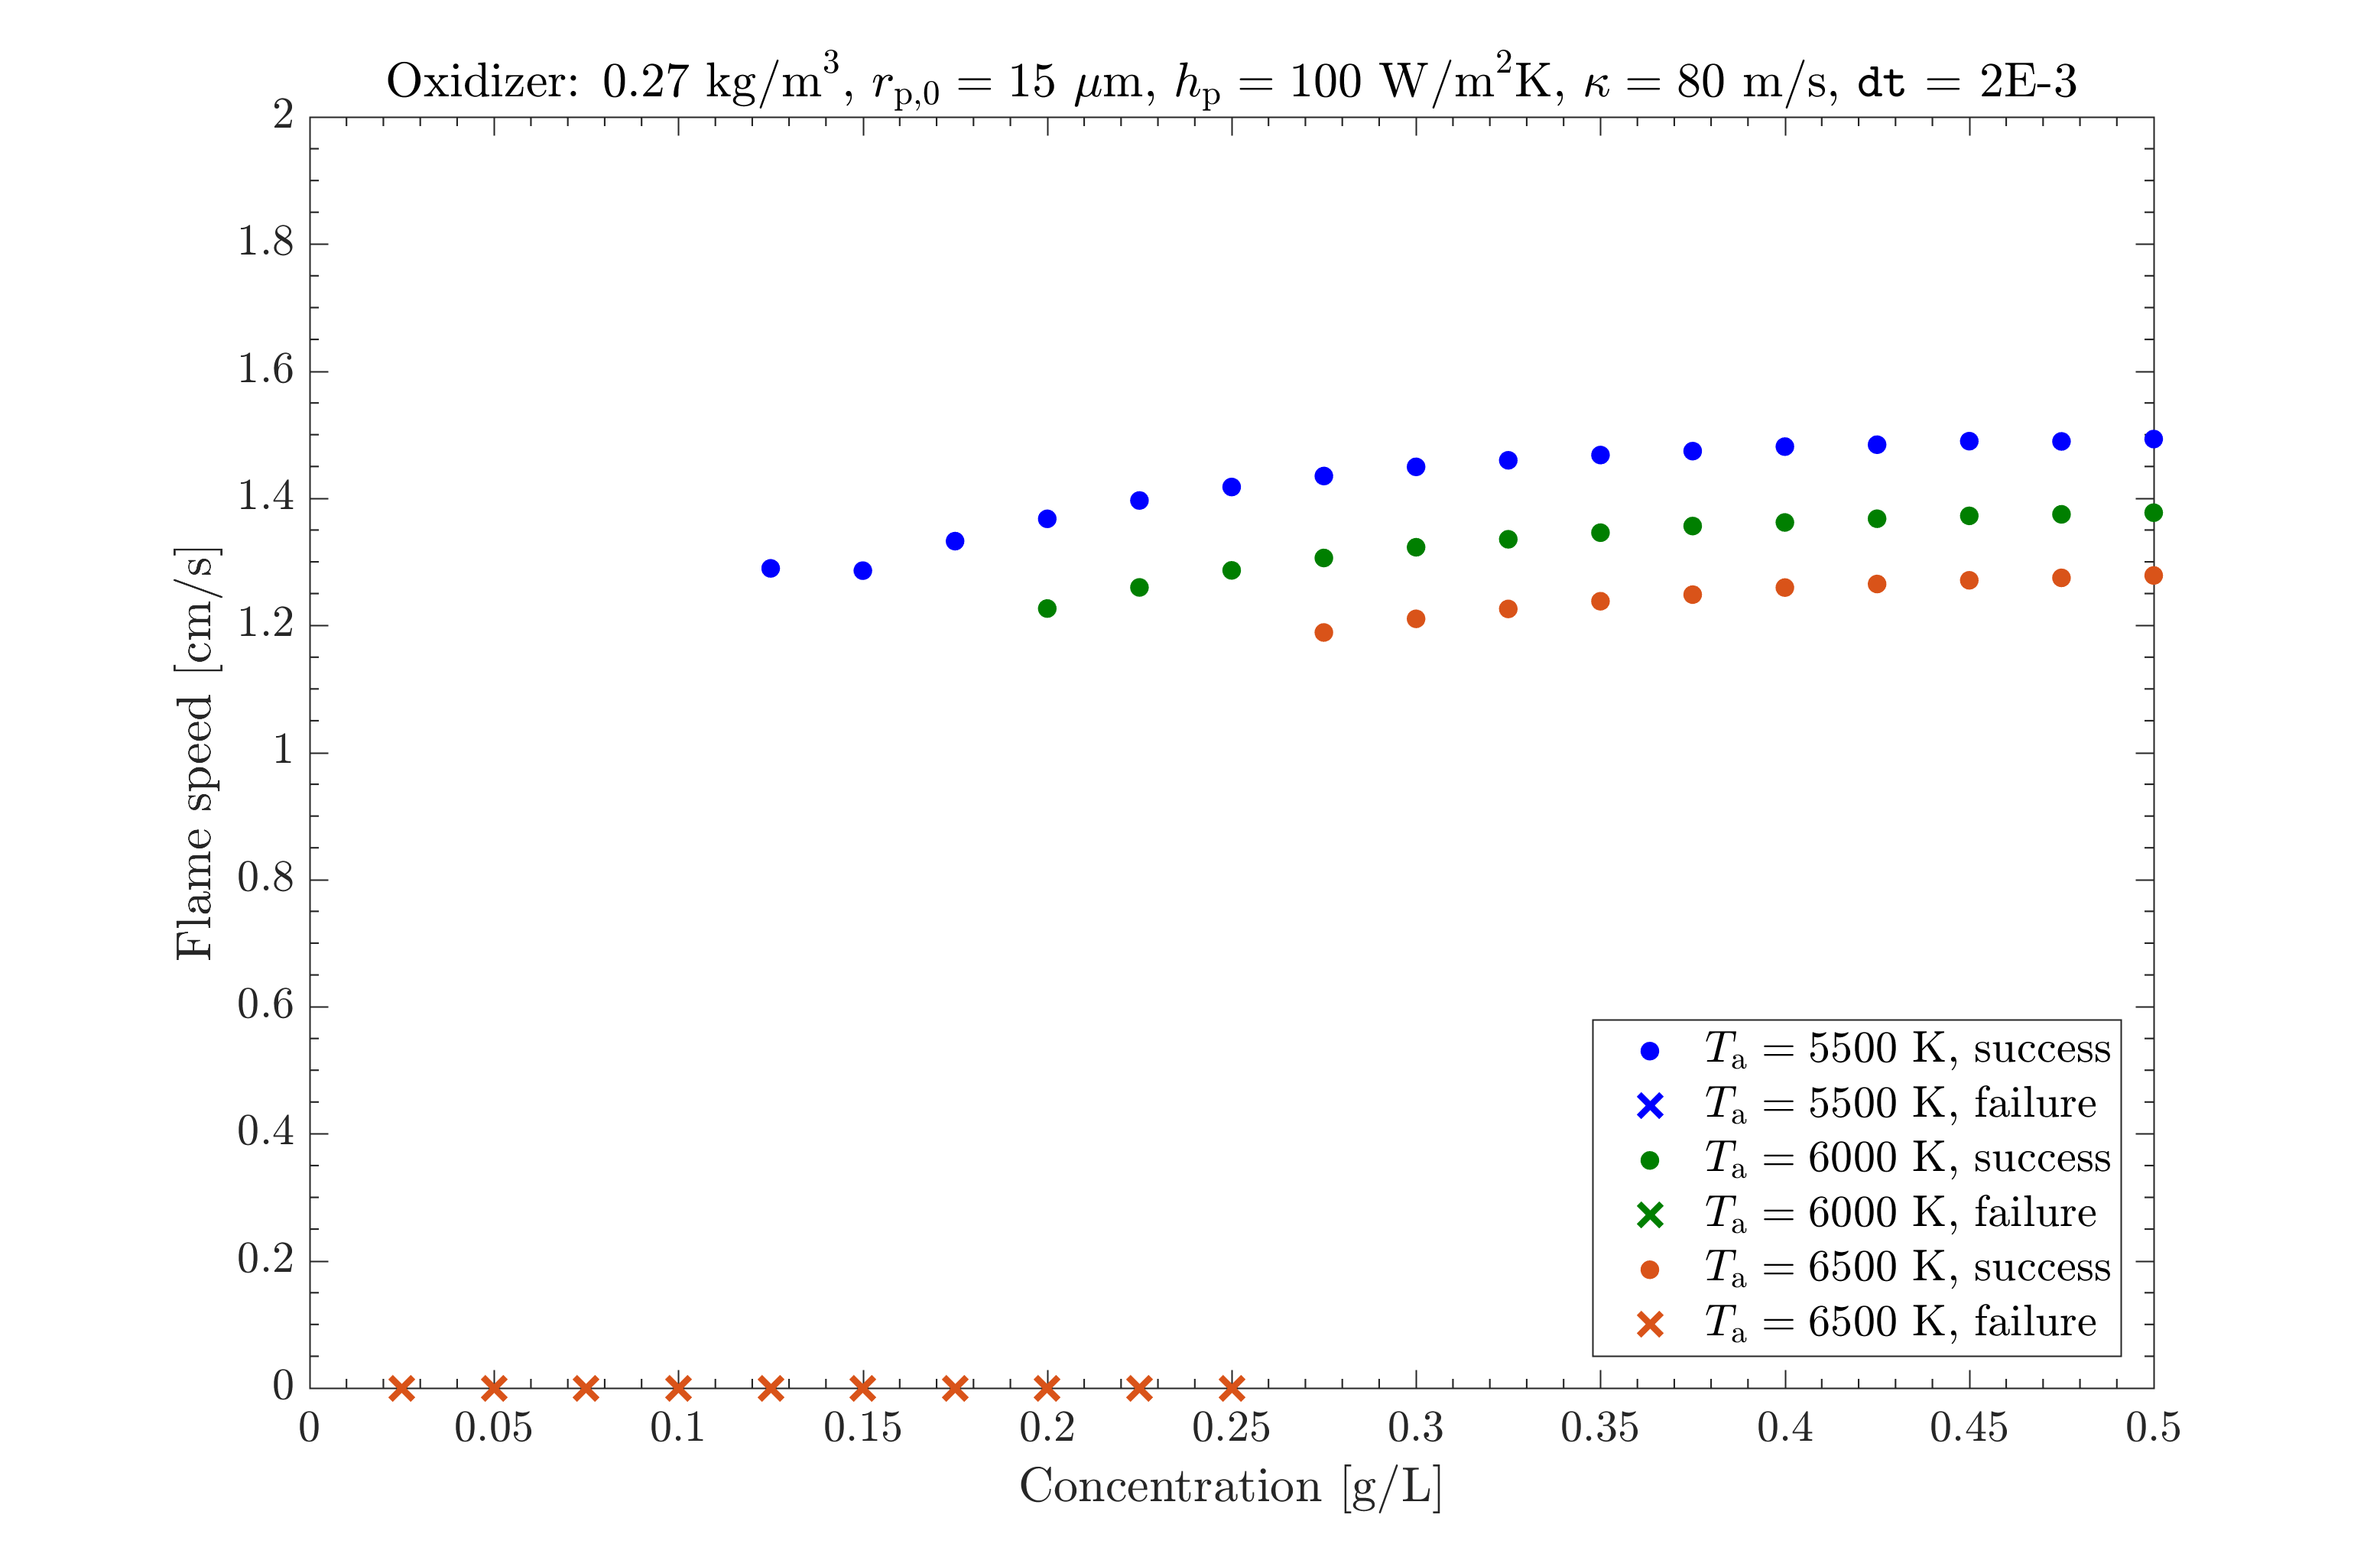
\includegraphics[width=\textwidth]{./Data/runSet1.png}
    \caption{Flame speed as a function of oxygen concentration for various activation temperature parameters. Other parameters are specified at the top of the plot box. X-markers (stacked one atop another) denote failure to propagate.}
    \label{fig:runSet1}
\end{figure}

\begin{figure}
    \centering
    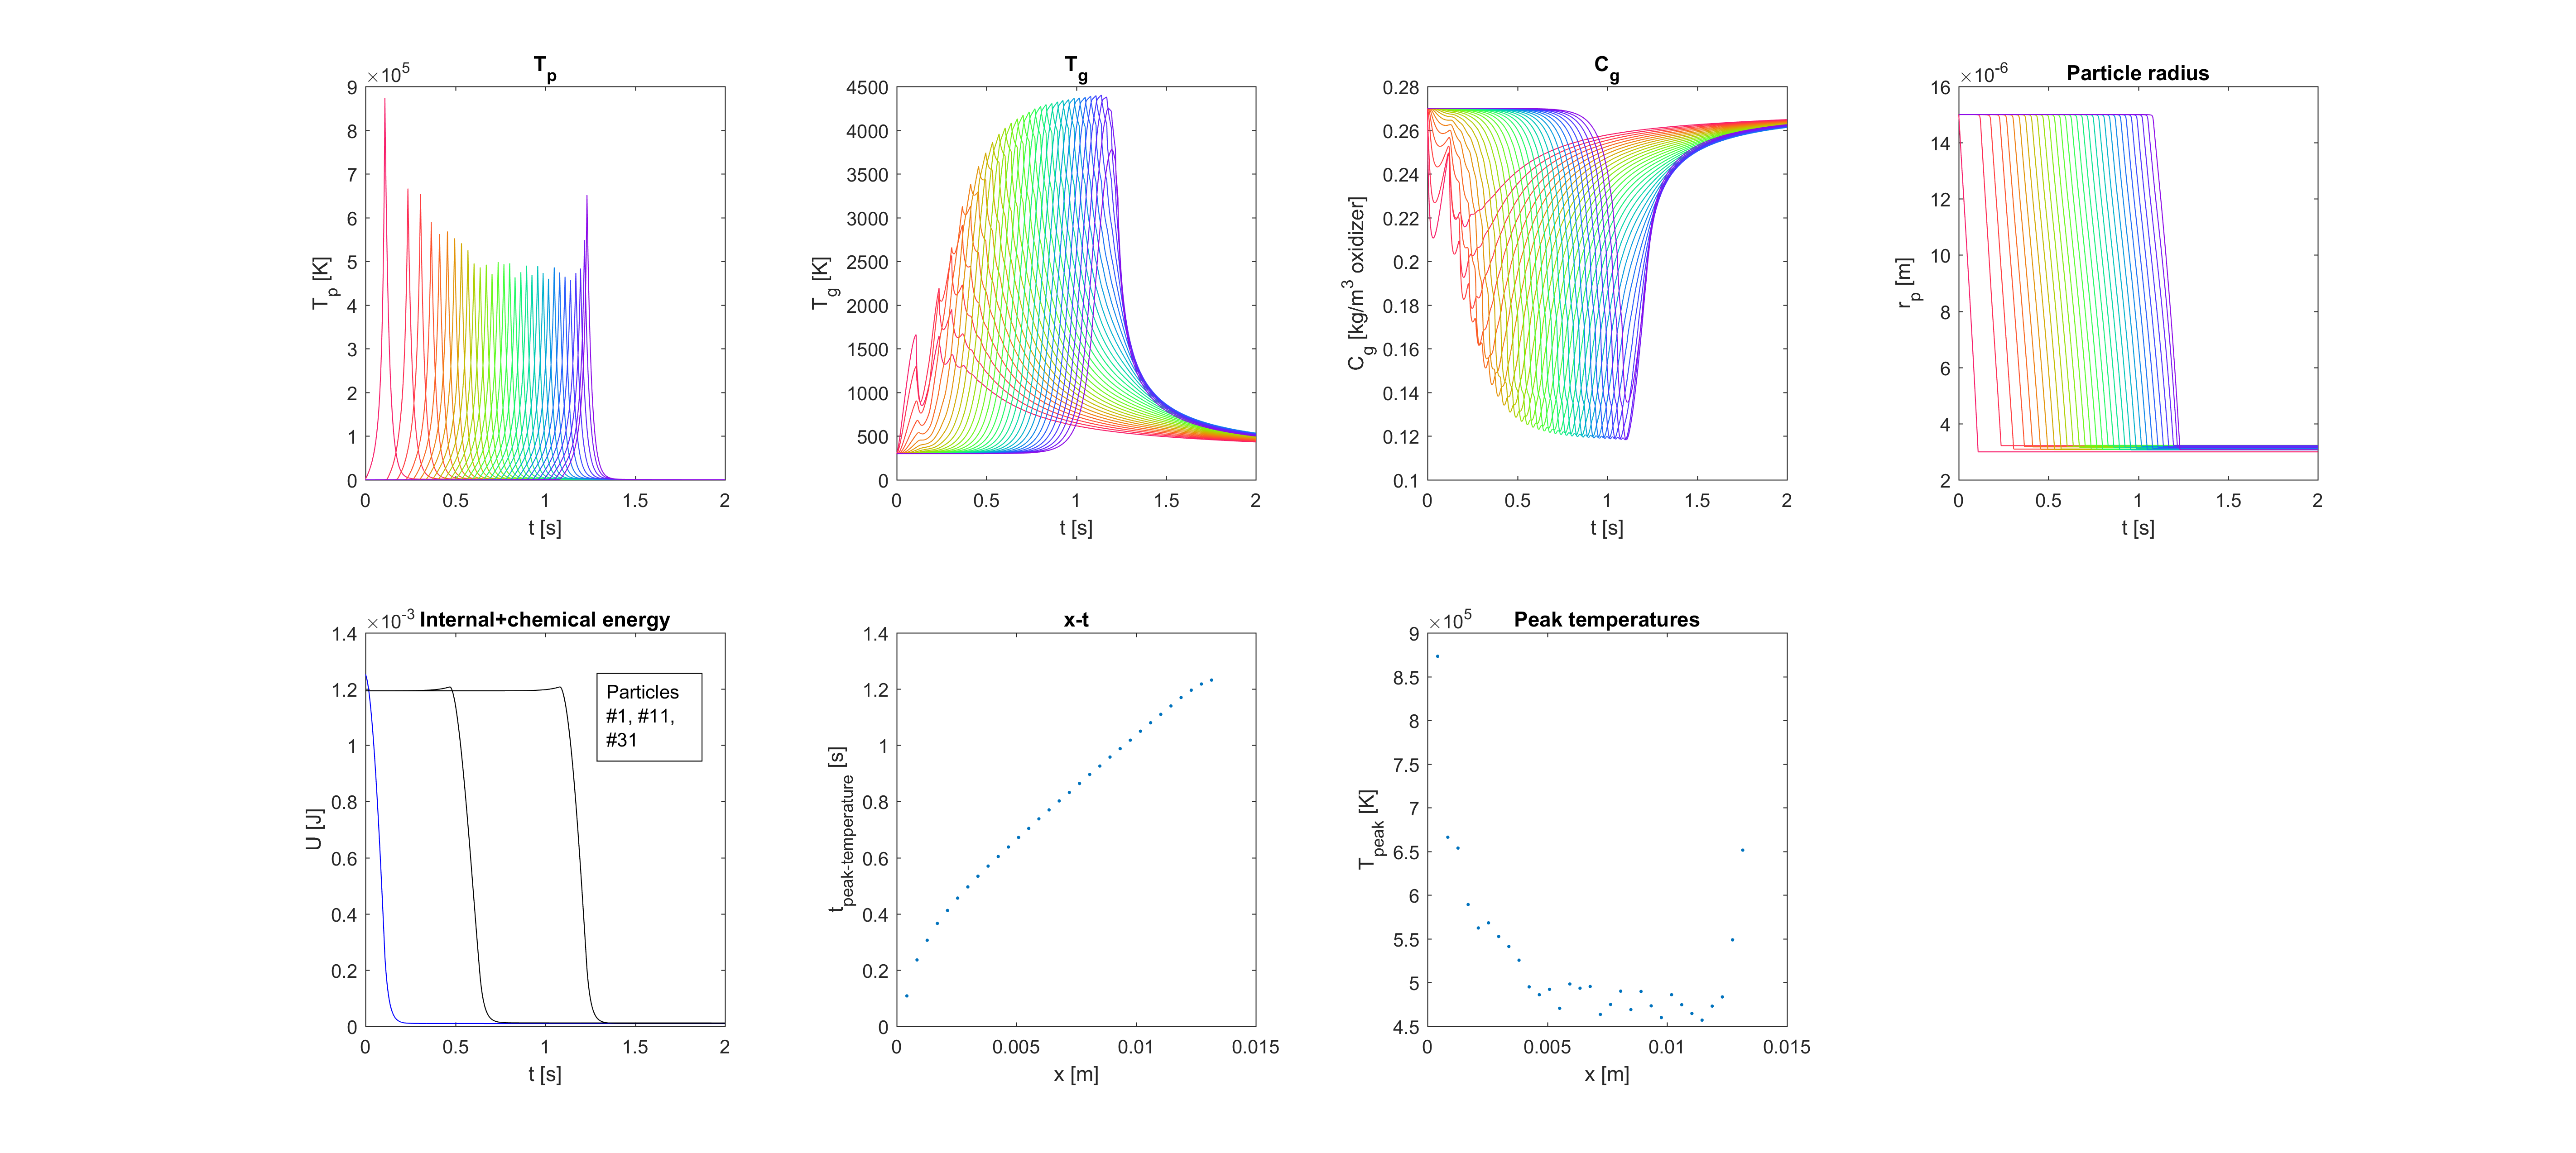
\includegraphics[width=\textwidth]{./Data/kb_outputSample_73.png}
    \caption{Debug dashboard containing some useful checks for a particular run of the model.}
    \label{fig:dashboard}
\end{figure}

\section{More on numerics of PDE}
\label{sec:morenumerics}

This is a technical section describing more how and why behind the numerical methods. Consider again the temperature-only PDE
\begin{equation}
    \frac{\partial T}{\partial t} - \nabla^2 T = \sum_{i=1}^{N_\mathrm{particles}}\delta(x-x_i) T(x,t)
\end{equation}
where we try to solve by approximating the convolution
\begin{equation}
    T^* = \int_0^t \sum_{i=1}^{N_\mathrm{particles}} G(\mathbf{x}-\mathbf{x_i},\tau) T(\mathbf{x}, t-\tau) d\tau
\label{eqn:fulltoy}
\end{equation}
which was inspired by the same strategy for an equation with an explicit right-hand side, i.e., without $T$.

\subsection{Did the method converge?}
A convergence to a similar finite-difference model was obtained at quite roughly $\mathcal{O}(\Delta t^\frac{1}{2})$. Convergence is also obtained for Arrhenius. Finite-difference modeling was performed using a smoothed boxcar function that approaches a discrete Dirac delta. Adiabatic walls are used with domain length $L = 10$, and four particles at $x = 2, 4, 6, 8$.

\subsection{Why the strange one-half convergence?}
A difficulty with this model is the mix of PDE and ODE, especially when we decide to write our PDE as an integral equation, i.e., Eqn. \ref{eqn:fulltoy}.

The integral equation is in a sense something we want to solve globally, while ODEs with initial values are something we want to solve by timestepping. By globally we mean that we want $T(t = t^*)$ to be determined as a function of $T(t < t^*)$ at previous times, so it makes sense that we should be able to update the $T( t < t^*)$ at previous times to get a better answer at time $t^*$. In fact, if we only had to deal with this integral in the wild, we would probably try to use a fixed point iteration (see Banach fixed point theorem), which proceeds as follows:

\begin{enumerate}
    \item Pick some reasonable $T_0$.
    \item Define the operator $A$ by $AT = \int_0^t K(\mathbf{x}, t, \tau) T(\mathbf{x}, \tau) d\tau$ where $K$ here is the sum of Green's functions in Eqn. \ref{eqn:fulltoy}.
    \item For the desired interval $[0,t]$, fixing $\mathbf{x}$, iterate $T_{k+1}(\mathbf{x}, t), = AT_k(\mathbf{x}, t)$ until (hopefully) $T_{k+1}$ is converged to $T^*$. The converged $T^*(\mathbf{x}, t)$ is then a function of $t$ at a fixed $\mathbf{x}$.
\end{enumerate}

Then in this case, we are allowing $T$ to change globally (in $t$), and the accuracy of the converged result depends on the $\Delta t$ with which we approximate the integral.

What's stopping us from going ahead and doing this is the ODE part of the model, for which it is more natural to use a timestepping strategy. We thus set in stone the previously computed gas temperatures $T_\mathrm{g}$ so we don't have to recompute the ODEs. The price we pay is we can't get the full convergence order on $T$ from the PDE.

\end{document}

